\chapter{Optical and Electronic Properties of Single-Wall Carbon Nanotubes}

\section{Introduction}
{\color{red}UNFINISHED} Carbon nanotubes are 1-D structures meaning that electrons are confined in a single dimension. They exist in terms of many chiralities, some are semiconducting and others are metallic \cite{soavi2016ultrafast}. Interesting because they let us explore the physics of 1-D structures. Due to the higher degree of confinement with respect to convention 3-D structures, different phenomena may occur.



\section{Carbon Nanotube Chiralities}

Carbon nanotubes are basically rolled up graphene sheets. Countless ways of rolling up a graphene sheet into cylindrical structures. Hence, nanotubes described using so-called chiral vectors. 

\begin{figure}[H]
	\centering
	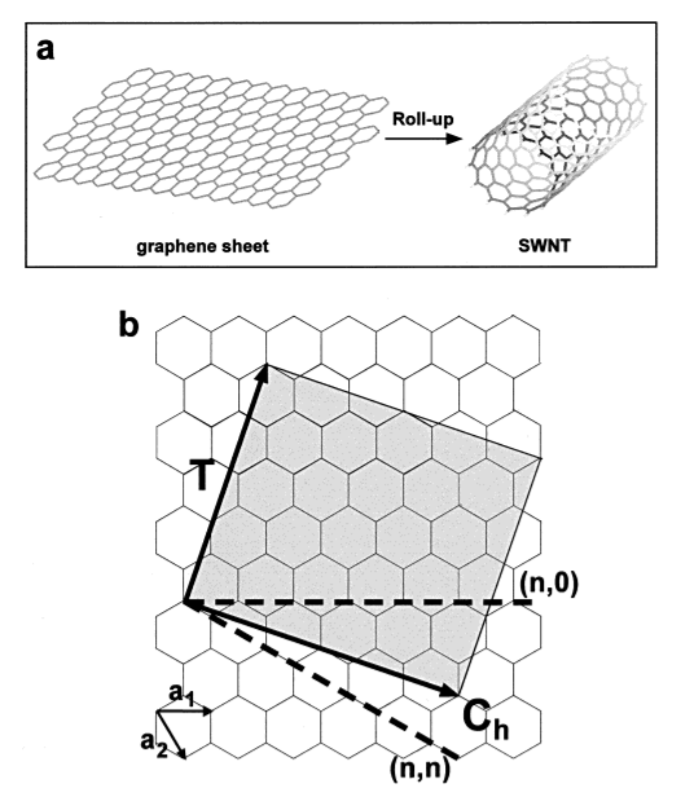
\includegraphics[scale=0.7]{images/chapter_optical_props/chiral_vectors.png}
	\caption{Figure of carbon nanotube bandstructure. Arrows drawn in figure to show allowed transitions. Reproduced from \cite{odom2000structure}.}
	\label{fig:chiral_vectors}
\end{figure}


\section{Optical Selection Rules}
\begin{itemize}
	\item Selection rules dictate which transitions can occur in the presence of certain conditions
	\item light polarized parallel to carbon nanotube excites one type of transition
	\item light polarized perpendicular to carbon nanotube excites another set of transitions
\end{itemize}

\begin{figure}[H]
	\centering
	\begin{subfigure}{\textwidth}
		\centering
		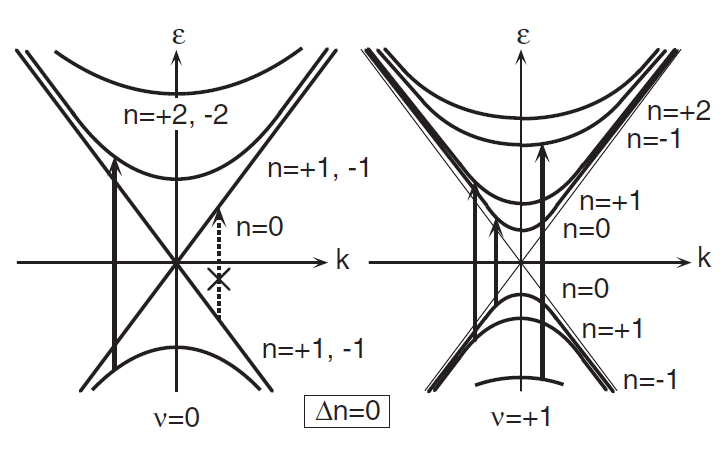
\includegraphics[scale=0.7]{images/chapter_optical_props/selection_rules_1.png}
		\caption{Selection Rules for Parallel case.}
	\end{subfigure}
	\begin{subfigure}{\textwidth}
		\centering
		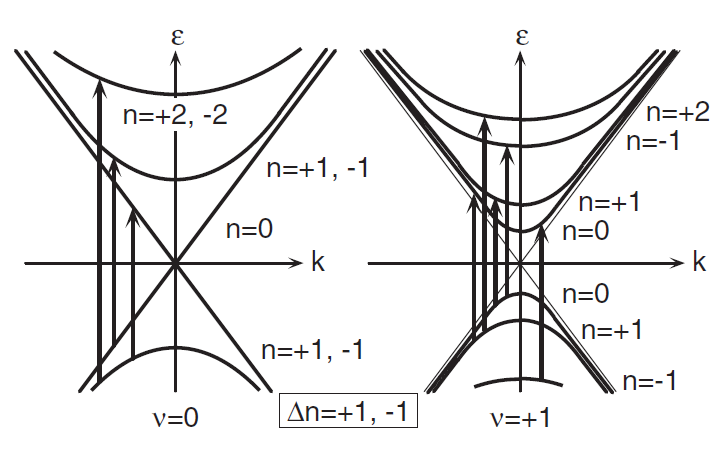
\includegraphics[scale=0.7]{images/chapter_optical_props/selection_rules_2.png}
		\caption{Selection rules for perpendicular case}
	\end{subfigure}
	\caption{Selection rules. Reproduced from Ref \cite{ando2005theory}.}
	\label{fig:selection_rules}
\end{figure}

\section{Excitons in Carbon Nanotubes}
All optical excitations in carbon nanotubes lead to direct creation of excitons \cite{wang2005optical}.

Due to strong quantum confinement, binding energy of Excitons in 1-D structures expected to be infinite \cite{ando2005theory}. This explains why nanotubes have such high exciton binding compared to 2-D and 3-D materials. 
 
\begin{figure}[h]
	\centering
	\includegraphics[scale=0.7]{example-image-a}
	\caption{Figure of GaAs absorbance at low-T and high-T to show weak binding energy of excitons. Next to this is a figure of  (6,5) absorbance at room temperature}
	\label{fig:gaas_vs_cnt_absorbance}
\end{figure}
